\section{\review{Optics Measurements}}
\label{section:opticcs_meas}

To perform optics measurements, several tools and techniques are used. This section details the
various implemented methods to measure specific observables.

% ===============================
%            Software
% ===============================
\subsection{\review{Tools and Softwares}}

In order to perform the measurements, analysis and simulations presented in this thesis, various
tools and softwares have been developed, used and contributed to.

Optics simulations have been done mainly in MAD-X~\cite{deniau_mad-x_nodate} and PTC.
MAD-NG~\cite{deniau_mad-ng_2020} and
Xsuite~\cite{g_iadarola_xsuite_nodate} have also been explored for specific tasks such as free RDT
simulations and GPU tracking.

Analysis of chromaticity measurements are done via a newly developed graphical
interface~\cite{m_le_garrec_non-linear_2022} written in Python. This tool makes cleaning of the raw
signal data, its analysis and results export more reliable and easier.
Overall, analysis of turn-by-turn measurements is supported by a large panel of libraries written by
the Optics Measurements and Corrections (OMC) team, in Python and Java~\cite{OMC-TeamPyLHCv0.3.0}.

%\begin{itemize}
%    \item \textbf{Beta-Beat GUI}~\cite{omc-team_beta-beat_2008}, Graphical interface for
%    turn-by-turn measurements visualization and analysis.
%    \item \textbf{OMC3}~\cite{omc-team_omc3_2021}, Main optics analysis and corrections software.
%    \item \textbf{Beta-Beat.src}~\cite{omc-team_beta-beatsrc_2018}, Old analysis software, now
%    replaced by OMC3.
%    \item \textbf{pylhc.github.io}~\cite{omc-team_omc_2020}, Website of the OMC team with package
%    documentation, examples and useful resources.
%\end{itemize}


% ===============================
%           TbT Data
% ===============================
\subsection{\review{Turn-by-Turn Signal}}

One of the key data acquisition methods for optics measurements in the LHC is turn-by-turn
acquisition, where beam position is collected on a per-turn basis. This process involves exciting
the beam using an AC-Dipole to induce forced oscillations. Typically, a pilot bunch is used for
this purpose, containing a reduced intensity of $10^{10}$ protons, compared to the standard
operational bunch intensity of $10^{11}$. The lower intensity allows for larger amplitude
oscillations, enabling more precise measurements while ensuring the safety of the machine and
minimizing the risk of damaging components.

A spectral analysis is then performed via a \textit{FFT} on the signal, making apparent the driven
tunes from the AC-Dipole, the transverse tunes and the possible resonance lines, as shown in
\cref{fig:optics_measurements:tbt_data:spectrum}.

\begin{figure}[!htb]
    \centering
    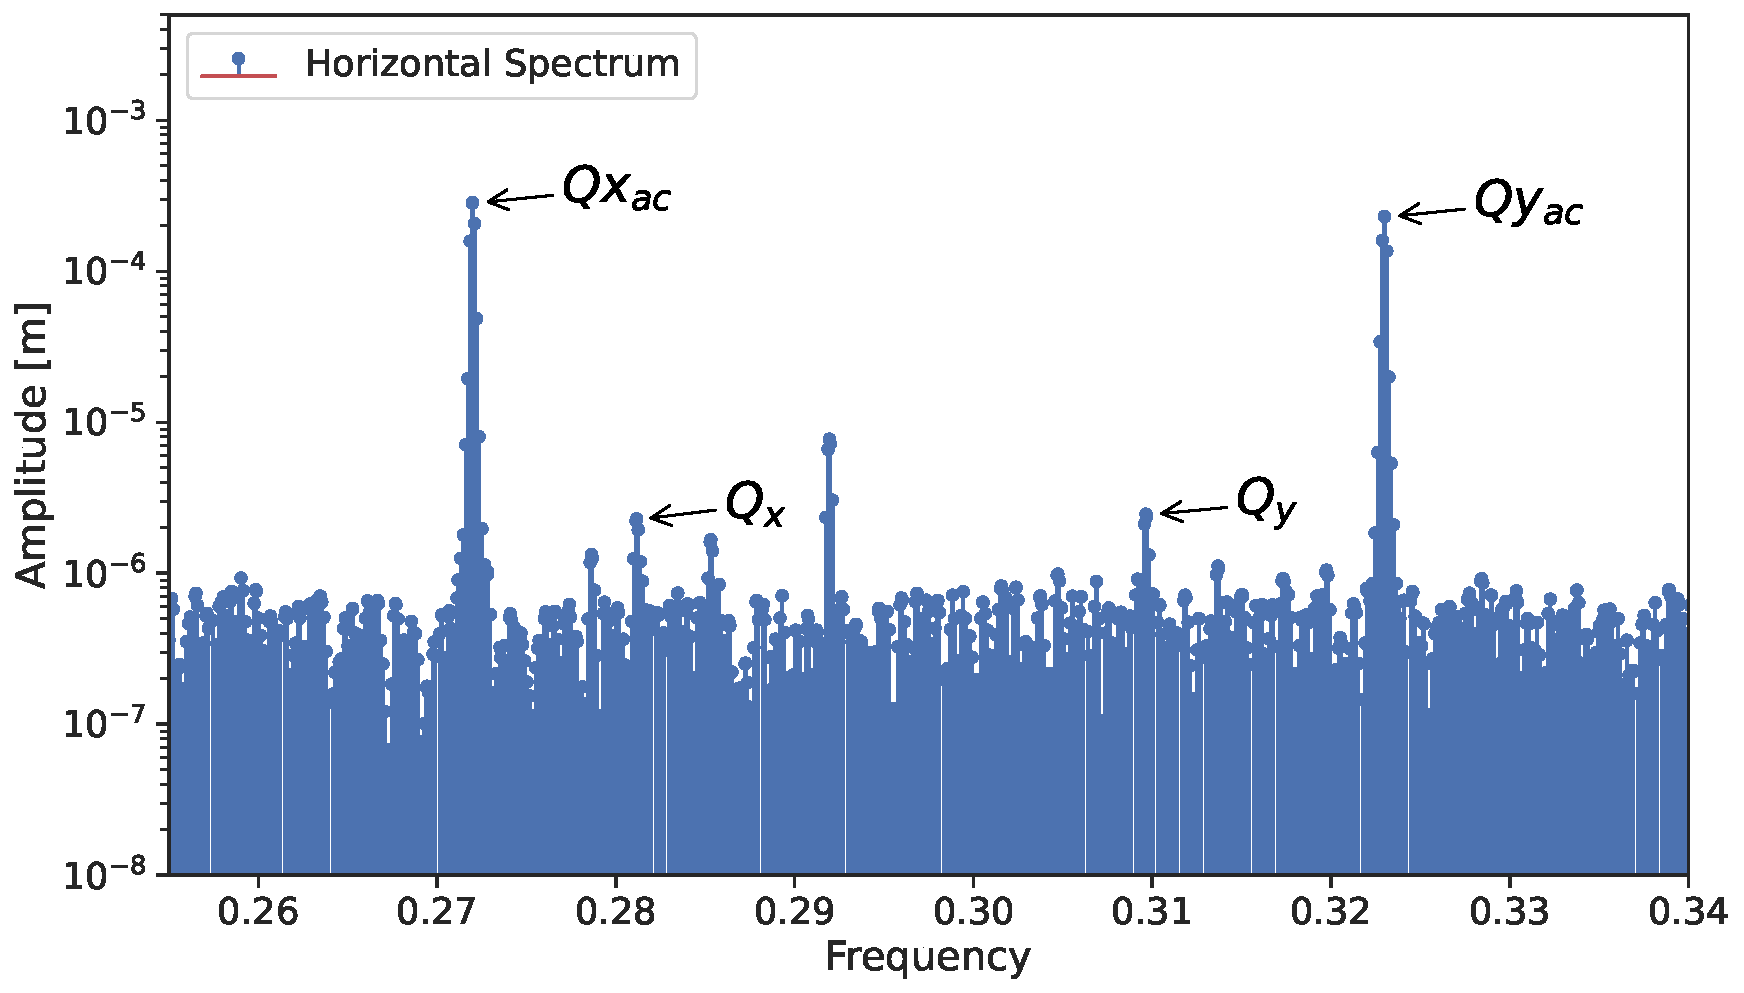
\includegraphics[width=0.8\textwidth]{./images/basic_spectrum.pdf}
    \caption{Horizontal frequency spectrum of a turn-by-turn measurement in the LHC. The 
    \textit{driven} tunes of the AC-Dipoles have the highest amplitudes while the natural tune can
    be seen close to it. Other lines are often created by resonances.}
    \label{fig:optics_measurements:tbt_data:spectrum}
\end{figure}

From these oscillations and  spectral lines, the optics observables, such as $\beta$-beating,
dispersion, coupling, and resonance driving terms, can be
reconstructed~\cite{catalan-lasheras_linear_2004}. These key quantities provide valuable insights
into the beam's dynamics and will be detailed further in the following sections.

\FloatBarrier

% ------- Betatron Phase
\paragraph{\review{Betatron Phase}}
The betatron phase can be determined at a given BPM by performing a FFT on the turn-by-turn
data. The argument of the retrieved complex number with the largest magnitude, the tune, is then
taken as the phase. The phase advance between two BPMs is simply their phase difference.


% ------- Beta Beating
\paragraph{\review{$\beta$-Beating}} 
The $\beta$-beating can be reconstructed via the phase advance between BPMs. The computation
involves using a model created via a simulation software such as MAD-X and makes use of transfer
matrices between elements. The $\beta$-function at a given BPM can be calculated from the
measured phases of 3 BPMs denoted $i, j, k$~\cite{minty_measurement_2003},

\begin{equation}
    \beta(s_i) = \beta^{model}(s_i) \cdot \frac{\cot(\Delta\phi_{i,j}) + \cot(\Delta\phi_{i,k})}{\cot\left(\Delta\phi_{i,j}^{model}\right) + \cot\left(\Delta\phi_{i, k}^{model}\right)}
\end{equation}

with $\Delta_{i,j}$ being the phase advance between BPMs $i$ and $j$. Using specific phase advances
between BPMs enhances the precision of the $\beta$-function measurement. This approach can also be
extended to use an arbitrary number $N$ of
BPMs~\cite{langner_utilizing_2016,wegscheider_analytical_2017}. The measurement of the
$\beta$-function via phase advance is independent from BPM calibration and relies solely on the
accuracy of the phase measurement.


% ------- Dispersion
\paragraph{\review{Dispersion}} To retrieve the linear dispersion, turn-by-turn measurements are
performed at certain momentum offsets. This allows the computation of the dispersion via the shift
in mean orbit $\Delta z$ and the momentum offset $\delta$,

\begin{equation}
    D_z = \frac{\Delta z}{\delta}.
\end{equation}

%In the LHC, measurements are typically taken at $\pm 100$Hz, corresponding to a momentum offset 
%$\delta \approx \mp0.7$.


% ------- Action
\paragraph{Action} 
The action in a given plane and BPM, located at position $s$ is calculated from the amplitude
$\mathcal{A}$ of the main peak in the frequency spectrum, which corresponds to the tune, along with
the beta-function at that BPM derived from the model,

\begin{equation}
    2J_{BPM} = \frac{\mathcal{A}_{BPM}^2}{\beta_{model,BPM}}.
\end{equation}

This method of action computation is directly influenced by BPM calibration
errors~\cite{garcia-tabares_valdivieso_optics-measurement-based_2020}. The overall action is then
the average over $N$ BPMs:

\begin{equation}
    2J = \frac{1}{N} \sum_n^N \frac{\mathcal{A}_n^2}{\beta_{model,n}}.
\end{equation}


% ------- Coupling
\paragraph{\review{Transverse Coupling}}

Coupling can be calculated by comparing the amplitude of the tune in the frequency spectrum of a
plane to the same tune in the other plane. The coupling RDTs $f_{1001}$ and $f_{1010}$ can be
reconstructed with these amplitudes~\cite{franchi_computation_2010,tomas_cern_2010},

\begin{equation}
    \begin{aligned}
        |f_{1001}| &= \frac{1}{2} \sqrt{\frac{H(0,1)V(1,0)}{V(0,1)H(1,0)}}, \\
        |f_{1010}| &= \frac{1}{2} \sqrt{\frac{H(0,-1)V(0,-1)}{V(0,1)H(1,0)}},
    \end{aligned}
\end{equation}

where H and V refer respectively to the amplitude of a $Q_x, Q_y$ line in the horizontal and
vertical frequency spectrum. For instance, H(1, 0) is the amplitude of $Q_x$ in the horizontal
spectrum while H(0, 1) corresponds to $Q_y$ in the same spectrum. The phases of these RDTs is given
by,

\begin{equation}
    \begin{aligned}
        q_{1001} &= \phi_{V(1,0)}  - \phi_{H(1,0)} + \frac{\pi}{2}, \\
        q_{1010} &= \phi_{H(0,-1)} - \phi_{V(0,1)} + \frac{\pi}{2}.
    \end{aligned}
\end{equation}

The final expression of the coupling RDTs is then,

\begin{equation}
    \begin{aligned}
        f_{1001} &= |f_{1001}|e^{i\cdot q_{1001}},\\
        f_{1010} &= |f_{1010}|e^{i\cdot q_{1010}}.
    \end{aligned}
\end{equation}


% ------- Amplitude Detuning
\paragraph{\review{Amplitude Detuning}}
Amplitude detuning measurements in the LHC are usually taken with varying AC-Dipole kick amplitudes.
A linear function is then fitted on the natural tunes $Q_x$ and $Q_y$ versus the action of either
planes $2J_x$ or $2J_y$.


% ------- Resonance Driving Terms
\paragraph{\review{Resonance Driving Terms}}
Resonance Driving Terms are measured in the LHC with varying AC-Dipole kick amplitudes. The
amplitude of the resonance line of interest in the frequency spectrum can then be fitted to the
corresponding action dependence of the RDT, as detailed in
\cref{section:background:frequency_spectrum} and \cref{appendix:rdts}. As a reminder, the amplitude
of the RDT will be given by,

\begin{equation}
    \begin{aligned}
    |f_{jklm}| &= \frac{|H_{f_{jklm}}|}{2 j (2 I_x)^\frac{j+k-1}{2} (2 I_y)^\frac{l+m}{2}} \\
    |f_{jklm}| &= \frac{|V_{f_{jklm}}|}{2 l (2 I_x)^\frac{j+k}{2} (2 I_y)^\frac{l+m-1}{2}} .
    \end{aligned}
    \nonumber
\end{equation}

The phase of the RDT can then be reconstructed via the momentum and phase advances. In practice,
\textit{forced resonance driving terms} are actually measured, as the oscillations are driven by
the AC-Dipole. Simulations are thus always made via tracking with an AC-Dipole to match.
Studies linking \textit{forced} RDTs to \textit{free} RDTs is though ongoing to better understand
the machine without excitation~\cite{carlier_nonlinear_2020}.


% ------- Lifetime
\paragraph{\review{Lifetime}}

The beam lifetime is a measure of how long the beam can remain circulating without significant
losses of particles. It is typically expressed in hours and is related to the rate
at which particles are lost from the beam. Particles might be lost due to resonant conditions,
instabilities or vacuum quality. The beam intensity is measured via the BCTs. The lifetime $\tau$
relates then the number $N$ of particles at a time $t$ to its rate of change,

\begin{equation}
    \tau = N(t) \cdot \frac{\diff N}{\diff t}^{-1}.
\end{equation}

Additionally, Beam Loss Monitors (BLMs) provide local information about beam quality by detecting
and localizing particle losses. These losses can as well be integrated to give a lifetime estimate.
At injection energy in the LHC, the beam lifetime with a pilot bunch is typically around 3 hours.
Sudden particle losses can significantly reduce the measured lifetime, even if the remaining beam
stabilizes and does not lose particles as rapidly. This introduces challenges in accurately
measuring the lifetime, as the signal needs to stabilize and saturate after any trim to ensure
reliable data.


% ===============================
%          Chromaticity
% ===============================
\subsection{\review{Chromaticity}}
\label{subsection:optics_corrections_chromaticity}

%% --- Procedure ---
%\subsubsection{\review{Procedure}}

Chromaticity measurements are performed by varying
the RF frequency to induce a change of momentum offset $\delta$, while measuring the tune. The
momentum offset $\delta$ being related to the RF frequency, the Lorentz factor $\gamma$ and the
momentum compaction factor $\alpha_c$~\cite{keintzel_jacqueline_beam_2022}:

\begin{equation}
    \delta = - \left(\frac{1}{\gamma^{-2} + \alpha_c}\right) \cdot \frac{\Delta f_{\text{RF}}}{f_{\text{RF,nominal}}}
    \label{eq:dpp_rf}
\end{equation}

In the LHC, the Lorentz factor $\gamma^{-2}$ is here negligible, as the energy is large even at
injection.  At 450 GeV, $\gamma^{-2} \approx 10^{-6}$, which is two orders of magnitude smaller than
$\alpha_c$.

During operation, where the linear chromaticity often needs to be measured, a sinusoidal function
with a period of $\approx 20$ seconds is applied on the RF frequency. This induces a change of
momentum offset to measure the first order of the chromaticity function, via a harmonic
fit~\cite{fuchsberger_ibic_2016}. For non-linear measurements, a large range of momentum offset is
required. In order to do so, a new procedure has been developed. Dense frequency scans with steps of
20Hz every 30 seconds are usually taken to compromise between number of data points, precision of
the tune estimate, and duration of the measurement. Once beam losses, registered by the BLMs are
deemed too high, the frequency is reverted back to its nominal value in larger steps. Attaining the
limits of the BLMs ensures a large momentum-offset range. The same procedure is then re-applied in
the negative.
\Cref{fig:measurements:rf_scan} shows a typical RF scan performed to measure non-linear chromaticity
in the LHC.

\begin{figure}[H]
    \centering
    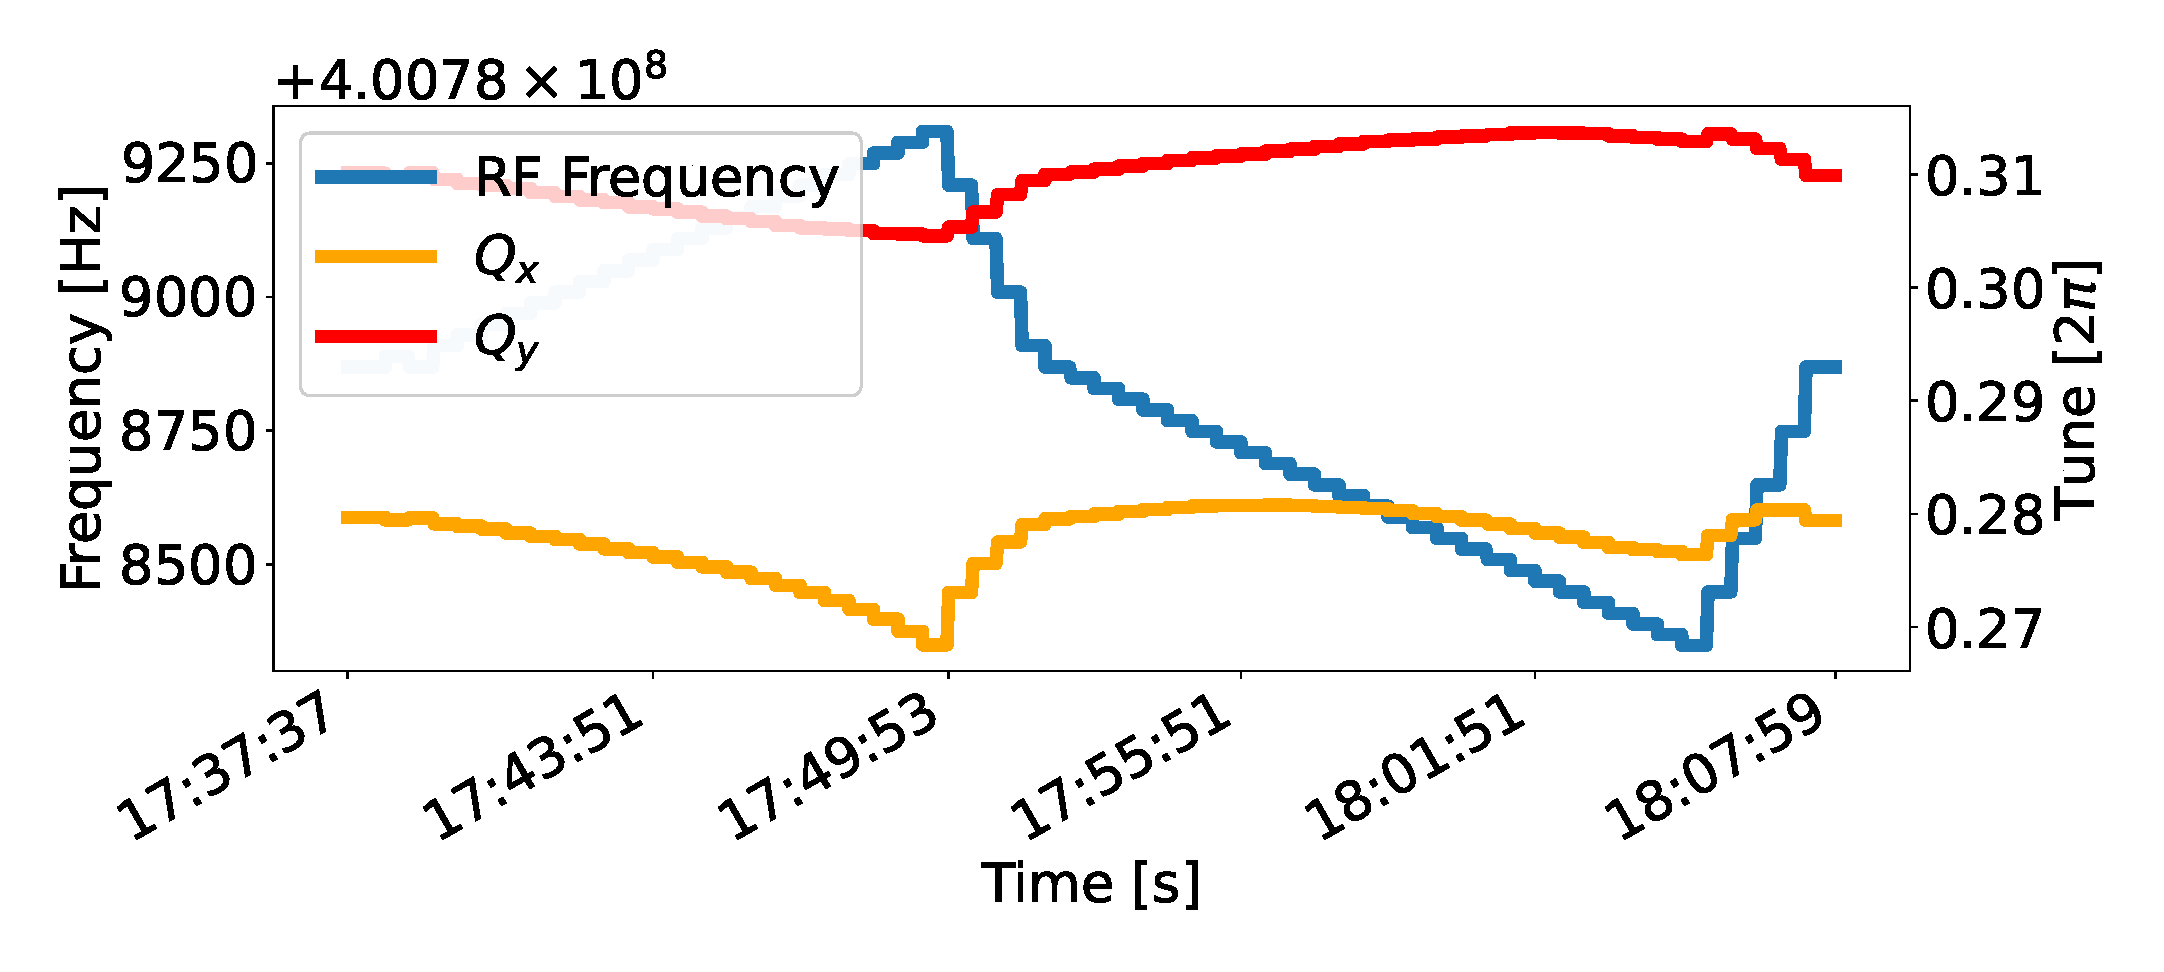
\includegraphics[width=1\textwidth]{images/rf_scan.pdf}
    \caption{Observation of the tune dependence on momentum offset, created by a shift of RF
             frequency.}
    \label{fig:measurements:rf_scan}
\end{figure}


%% --- Analysis and Fit ---
%\subsubsection{\review{Analysis}}

Once the tunes have been acquired and the momentum offset computed via \cref{eq:dpp_rf}, the
chromaticity function (see \cref{eq:background_chromaticity}) can be used to fit the
measured data and retrieve each order.

As part of the work for this thesis, a new tool, was developed. in order to ease and improve the
analysis of chromaticity measurements. 
The Non-Linear Chromaticity GUI~\cite{m_le_garrec_non-linear_2022} showcases new analysis techniques
using the raw signal from the BBQ system along with custom signal cleaning that are detailed later
on in \cref{chapter:high_order_fields}. Fits to very high chromaticity orders are also now possible
along with their computed corrections and that of Resonance Driving Terms via a combined response
matrix approach. Automatic data extraction from the CERN data servers (Timber, NXCALS) is also
included.
